
\subsection{Modalities}
Positive reinforcement rewards can be delivered using technology from different modalities. Visual, auditory and visual-auditory are the most methods for issuing feedback in HCI~\cite{desinging_interface_speech_tech}. Feedback from each of these different modalities has been shown to improve task performance for small tasks~\cite{chi_oussama_tap_the_shapetones}. Combining modalities can be useful for issuing user feedback, enabling systems to be accessible to varying ages~\cite{article_user_centred_multimodal_reminders}. Individual modes can improve the effectiveness of reminders~\cite{multi_modal_reminders_less_disruptive, article_designing_multimodal_reminders_for_home}. However, the effectiveness of each type of modality as reward feedback and how combined modalities affect interaction has little research. Therefore, technology to support behaviour change should explore a range of modalities and feedback should not be annoying as positive reinforcement should be a satisfactory experience. Research into visual, auditory and visual-auditory feedback was identified to understand how they impact behaviour to see how habit formation is impacted.

\begin{figure}[H]
  \centering
  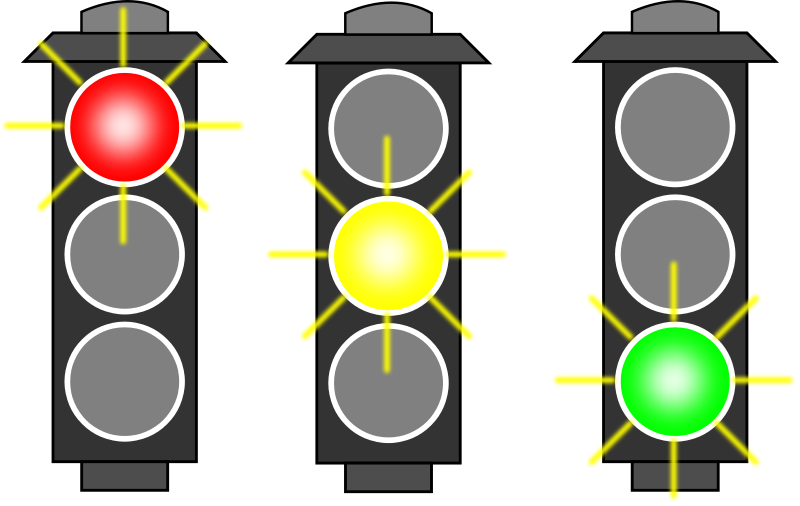
\includegraphics[width=2.6in]{../resources/visual.png}
  \hspace{10px}
  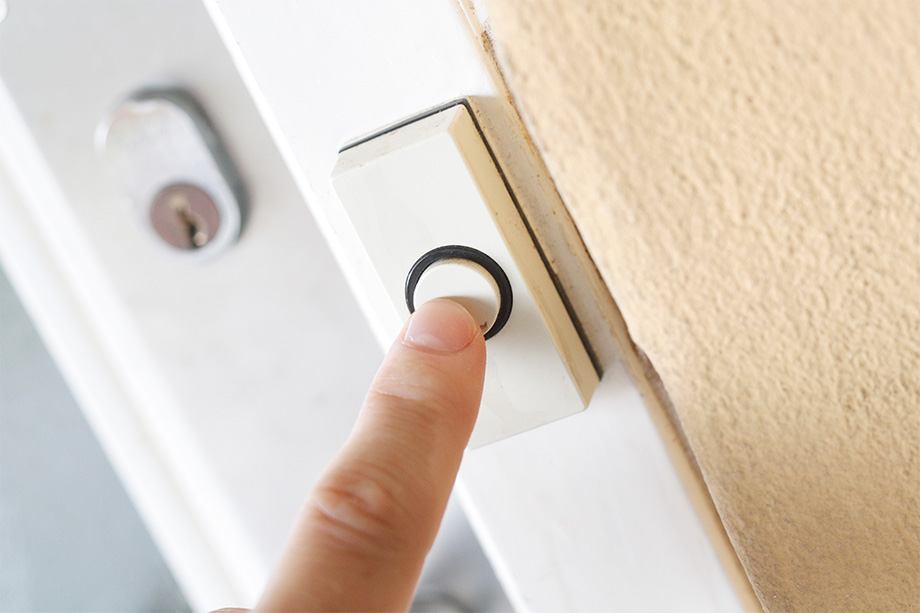
\includegraphics[width=2.6in]{../resources/audio.png}
  \caption{An example of visual (traffic light) and auditory (doorbell) feedback.}
  \label{fig:visual_audio}
\end{figure}

\subsubsection{Visual}
Visual feedback can encourage task performance consistency as demonstrated in one study by Lee et al.~\cite{article_realtime_feedback_improving_medication_taking} where they constructed a device that gave constant visual feedback for patients taking medication. They found that visual feedback improved consistency of the habit and increased the rate of self-efficacy. But when the device was removed, their performance dropped (as measured after a 2-month period). This suggests that users did integrate the visual feedback display cue with their routines, but they also became dependant on the technology and the visual feedback did not build habit strength. Users should instead build these cues outside of the system, with another routine to build habit automaticity and allowing for permanent behaviour change after the system is removed.

\subsubsection{Auditory}
There is a need to use audio when designing for behaviour change technology, especially with a varied target market~\cite{article_designing_for_health_behaviour_change_hci}. For example, combining different sounds for different actions to suit different users~\cite{article_movipill_improving_medication_elders}. Using auditory as a method of delivery has shown to improve task success~\cite{auditory_notifications_increase_delivery_success}, but little work has shown how it impacts habit performance.


\subsubsection{Visual-Auditory}
Several studies show that combining audio with visual as feedback after the completion of a simple task, can be successful~\cite{benefits_of_audio_visual_1, benefits_of_audio_visual_2}. A meta-analysis of 43 multi-modal studies~\cite{comparing_modalities_effects_of_visual_auditory} revealed that it was the most effective to increase performance, when a single task is being performed and when compared with visual or auditory feedback alone. Additional research shows this combination of visual and auditory sensory channels has been shown to increase performance with complex tasks~\cite{chi_oussama_tap_the_shapetones}. However, care needs to be taken when adding an extra modality as this study showed that '\textit{visual feedback improved task performance, but sacrificed task quality}'~\cite{comparing_modalities_effects_of_visual_auditory}. In addition, while all modalities contribute to perceptual experience, one sense can override another if the sensory channel mediates less ambiguous information than the other~\cite{one_mode_override_another}. Therefore it will be useful to compare the success of the task with the other modes. Using a combination of modalities for interaction gives a means of communication to people with varying levels of sensory awareness.

\subsubsection{Tactile Vibration}
The majority of electronic activity monitors already use behaviour change techniques and therefore present a medium which tactile vibration behaviour change interventions could occur~\cite{benefits_of_audio_visual_1, article_designing_for_health_behaviour_change_hci}. A survey on activity monitors~\cite{article_wearable_good} ranked \textit{Fitbit} (\url{www.fitbit.com}) devices as good vehicles for behaviour change techniques. Therefore, the Fitbit, would be a good primary platform for integrating vibration for rewards. However, due to technical limitations, as discussed in Section~\ref{limitations_and_future_work}, we are unable to implement them.


